% begin module tangent-overview
\begin{frame}
\frametitle{The Tangent Problem}
\begin{columns}[c]
\column{.35\textwidth}
\ \uncover<4->{%
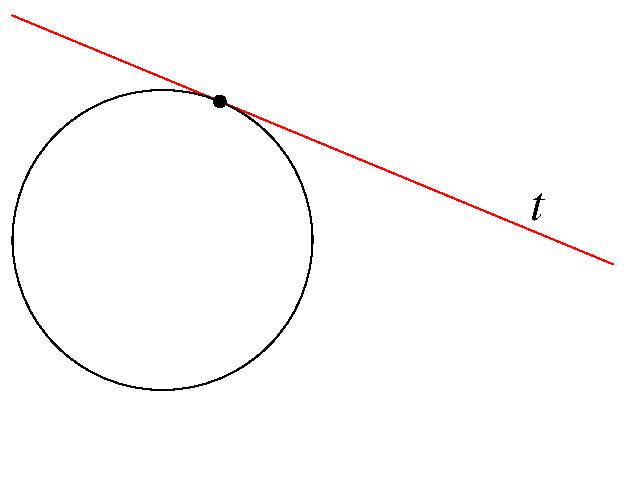
\includegraphics[height=3.5cm]{limits/pictures/02-01-tangenta.pdf}%
}%

\ \uncover<5->{%
\only<handout:0| -5>{%
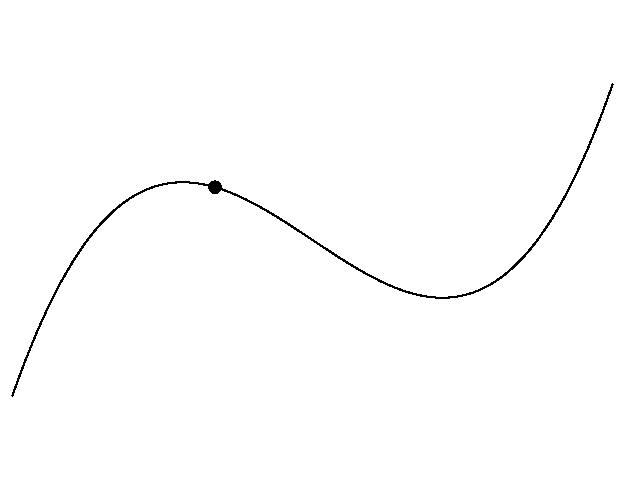
\includegraphics[height=3.5cm]{limits/pictures/02-01-tangentb.pdf}%
}%
\only<handout:0| 6>{%
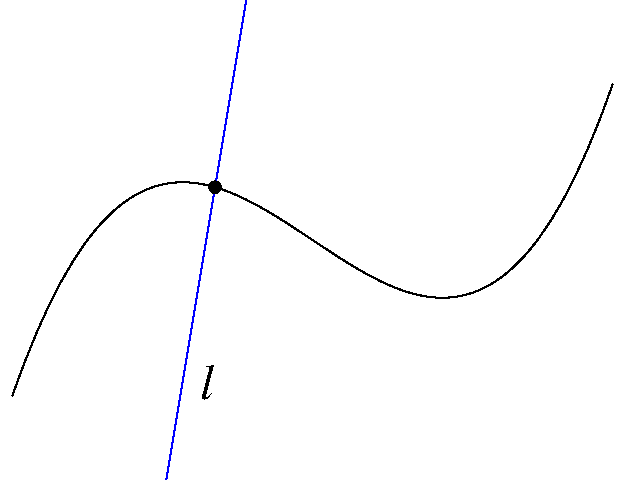
\includegraphics[height=3.5cm]{limits/pictures/02-01-tangentc.pdf}%
}%
\only<7->{%
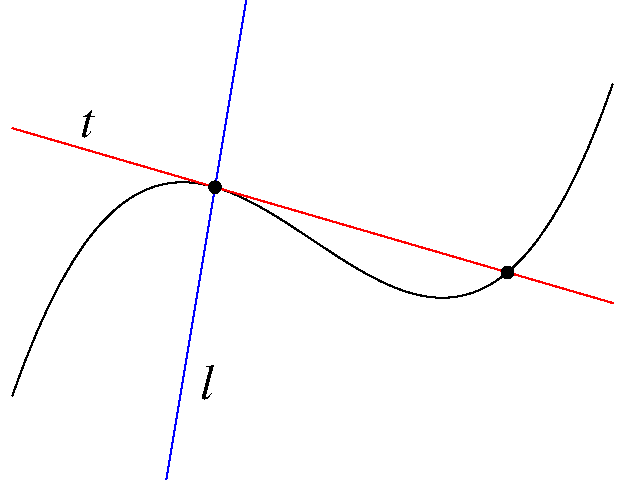
\includegraphics[height=3.5cm]{limits/pictures/02-01-tangentd.pdf}%
}%
}%
\column{.65\textwidth}
\begin{itemize}
\item<2->  A tangent is a line that touches a curve.
\item<3->  Moreover, a tangent should have the same ``direction'' as the curve at the point of contact.
\item<4->  For a circle, a tangent is a line that intersects the circle at exactly one point.
\item<5->  For more general curves, this definition isn't good enough.
\item<6->  The line $l$ intersects the curve at exactly one point, but it doesn't look like a tangent.
\item<7->  The line $t$ does look like a tangent, but it intersects the curve at two points.
\end{itemize}
\end{columns}
\end{frame}
% end module tangent-overview
